\chapter{System Design}
\vspace{-3mm}
The project was broken up into multiple stages, of which lead up to the design and manufacture of a PCB. This was used to create a list of goals that were required to be completed in order to successfully complete the project. This is also used to track the project progress in order to ensure that each stage of the project is accomplished in a timely manner.

\vspace{4mm}
\textbf{The project stages were:}
\begin{figure}[H]
\Centering
\begin{tabular}{l}
    1. Requirement Specification\\
    2. Design\\
    3. Component Testing\\
    4. Software\\
    5. PCB Design\\
    6. PCB Testing and Assembly\\
    7. Project Review\\
\end{tabular}
\end{figure}
\vspace{-7mm}
    
\section{Requirement specification}
The designed servomotor control board will need to have the following capabilities in order for it to be able to achieve the same functionality that devices such as the Dynamixel and other actuators can achieve. 

\vspace{7mm}
\textbf{The following functionality is required:}
\begin{table}[H]
    \centering
    \begin{tabular}{|c |c| c|}
    \hline
        \textbf{\underline{Control}} & \textbf{\underline{Communication}} & \textbf{\underline{Sensors}}\\
        Position  & UART  & Current\\
        Current & & Temperature\\
        \hline
    \end{tabular}
\end{table}
\newpage
\section{Hardware Design}
\vspace{-3mm}
An initial board layout based on the design specifications and requirements was created seen in Figure 3.1. This was used to determine all necessary components that would required. This is then also used when positioning the different components on the PCB.
\begin{figure}[H]
\centering
 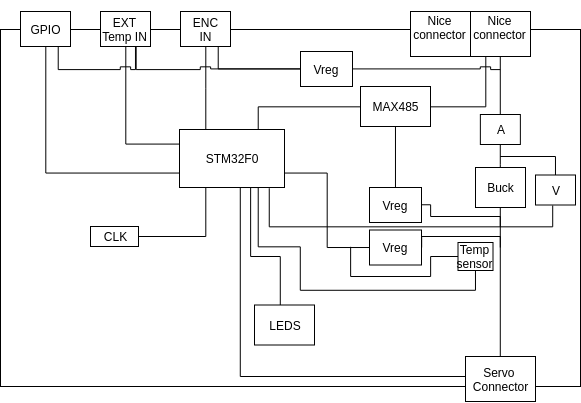
\includegraphics[width=0.58\textwidth]{My_board.png}
\caption{Basic board design}
\end{figure}  
\vspace{-7mm}
A flow diagram representing the two aspects of the system, power and communication can be seen in Figure 3.2.
\vspace{-2mm}
\begin{figure}[H]
\centering
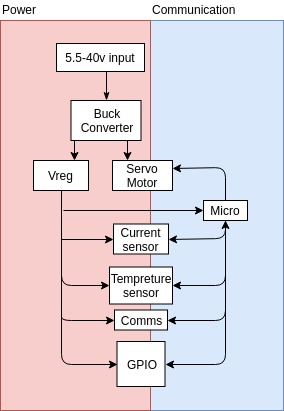
\includegraphics[width=0.45\textwidth]{System_Flow.jpg}
\caption{System flow diagram}
\label{fig:sysflow}
\end{figure}

\newpage
\section{Software Design}
The Slave microcontrollers will be programmed to interact with all its peripherals and perform communication using standard protocols. The Master microcontroller will control each Slave and be able to request information such as temperature and current drawn. A basic diagram of the interaction between the microcontroller and the code running on them can be seen in Figure 3.3.

\begin{figure}[H]
\centering
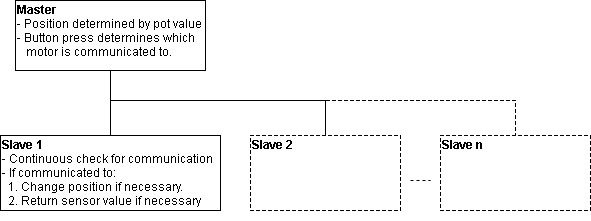
\includegraphics[width=0.9\textwidth]{Master_slave.jpg}
\caption{Master and Slave configuration}
\label{fig:masterslave}
\end{figure} 



\begin{figure}[H]
  \centering
  \begin{minipage}[b]{0.45\textwidth}
    \subsection{Master logic}
    The logic for the code running on master microcontroller can be seen in the diagram below in Figure 3.4.
    \vspace{2mm}
    \begin{figure}[H]
    \centering
    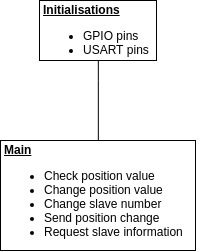
\includegraphics[width=0.8\textwidth]{Master_flow.jpg}
    \caption{Master code flow}
    \label{fig:MASTERFLOW}
    \end{figure} 
  \end{minipage}
  \hfill
  \begin{minipage}[b]{0.45\textwidth}
    \subsection{Slave logic}
    The logic for the code running on the slave microcontrollers can be seen in the flow diagram below in Figure 3.5.
    \vspace{5mm}
    \begin{figure}[H]
    \centering
    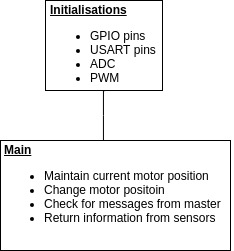
\includegraphics[width=0.9\textwidth]{Slave_flow.jpg}
    \caption{Slave code flow}
    \label{fig:SLAVEFLOW}
    \end{figure} 
  \end{minipage}
\end{figure}
\vspace{-5mm}

\newpage
\section{Component Selection}
After the system requirements have been established, and a basic system design has been created. The necessary components can be chosen.

The components that were chosen for the board had to be small enough to make the board compact, but still big enough so that it could be soldered down by hand accurately. Ideally a pick and place machine could be used to do the soldering, allowing for smaller components to be chosen, but for the sake of producing a functioning prototype it was only practical to choose slightly bigger components.


\subsection{Microcontroller}
The chosen micro controller needed to have the ability to interact with all the peripherals on the board as well as complete necessary computations in order for it to be able to control the servo motor board. As well as meeting the technical specifications, the chosen micro needed to be well documented in order to simplify the coding and debugging process.

The STM32F051C6 has an ARM Cortex-32-bit RISC core operating at up to 48MHz. This microcontroller was chosen as it met all the requirements and includes the following peripherals and functionality:
\vspace{5mm}
\begin{table}[H]
\centering
    \begin{tabular}{|c|c|}
    \hline
      \textbf{\underline{Features}} & \textbf{\underline{Types of communication}}\\
      64Kbytes of Flash & I2C \\
      12 bit ADC & SPI\\
      12-bit DAC & I2S\\
      six 16-bit timers & HDMI\\
      32-bit timer & USART\\
      Advanced control timer & \\
      Temperature sensor & \\
      \hline
    \end{tabular}
\end{table}
\vspace{-5mm}
The STM32F051C6 supports hardware controlled RS485 USART communication which will allow for the communication between the micro controllers using the MAX485 chip.
Its 12-bit ADC is a successive approximation analogue-to-digital converter. 

\newpage 
\vspace{5mm}
It has up to 16 channels which can be used to read the output voltage from the current and temperature sensors as well as from other GPIO pins. A 16-bit timer will be used to output the PWM signal the will be used to control the servomotors position.With multiple low power modes minimising the overall power consumption, optimising performance and consumption which is very important for applications that are run off batteries. 

\vspace{7mm}
In Figure 3.6, the necessary net labels were appended to the pins that are required for the microcontroller to function, as well as the pins that will be used to interact with the different peripherals.\vspace{2mm}
\vspace{10mm}
\begin{figure}[H]
\centering
\vspace{-5mm}
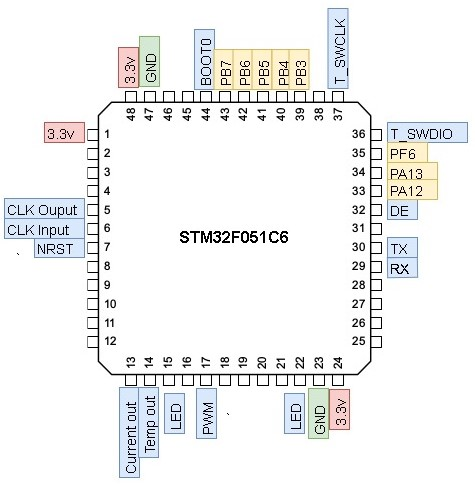
\includegraphics[width=0.6\textwidth]{micro.jpg}
\caption{STM32F051 LQFP48 package\cite{STM}}
\label{fig:STM}
\end{figure}
\vspace{1mm}
The STM will be programmed using the Atollic TrueSTUDIO IDE. The code was then compiled to hardware code and uploaded to the microcontroller using the ST-link debugger supported by Atollic.

\newpage
\subsection{Temperature sensor}
\vspace{5mm}
An analogue temperature sensor was chosen, the voltage output will be connected to one of the microcontrollers ADC. The MCP9700T has been designed for general purpose temperature monitoring and is typically used in home appliance and office equipment as well as hard disks and other PC peripherals.
\vspace{2mm}
\begin{figure}[H]
  \centering
  \begin{minipage}[b]{0.4\textwidth}
    \centering
    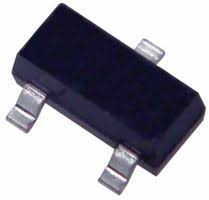
\includegraphics[width=0.4\textwidth]{MCP9700T.jpeg}
    \caption{MCP9700T chip \cite{MCP9700T} }
  \end{minipage}
  \hfill
  \begin{minipage}[b]{0.55\textwidth}
    \begin{table}[H]
      \centering
        \begin{tabular}{|l|}
        \hline
          \textbf{The MCP9700 has the following features:}\\
            - Input voltage range of 2.3V to 5.5V\\
            - Operates between -40\degree C to 125\degree C\\
            - 2\degree C accuracy between 0\degree C to 70\degree C\\
            - 10.0mV/\degree C resolution\\
            \hline
        \end{tabular}
        \caption{MCP9700 features}
    \end{table}
  \end{minipage}
\end{figure}
Unlike resistive sensors, the Linear Active Thermistor IC does not require any signal conditioning and the Vout pin should be directly connected to the input of a microcontroller.
The temperature coefficients are scaled to provide a 1\degree C/bit resolution for an 8-bit ADC with a reference voltage of 2.5V and 5V respectively.
This device is immune to the effects of parasitic capacitances which provides flexibility with the PCB layout as the device can be remotely located from the micro controller.

\begin{figure}[H]
  \centering
    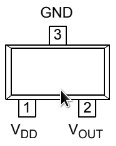
\includegraphics[width=0.15\textwidth]{MCP9700_setup.png}
    \caption{MCP9700 typical setup}
    \label{fig:model}
\end{figure}


\newpage
\subsection{Current sensor}
The chosen current sensor was the INA169 high side current shunt monitor. It is an analogue current sensor that produces and output current relative to that of a differential input voltage. The input voltage is read from either side of a current sensing resistor RS. The output current is then converted to a voltage across a load resistor RL. The voltage gain depends on the size of the Rl and thus can be controlled to have an output voltage of the same range as the input to the microcontrollers ADC. As a result the output can be connect directly to the input of the microcontroller ADC.

This type of  current sensor is typically used in automotive, computer and cellphone power management amongst other things. 
\begin{figure}[H]
  \centering
  \begin{minipage}[b]{0.4\textwidth}
    \centering
    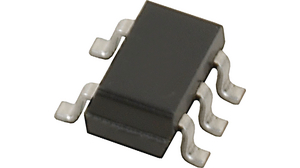
\includegraphics[width=0.5\textwidth]{INA169.jpg}
    \caption{INA169 chip \cite{INA169} }
  \end{minipage}
  \hfill
  \begin{minipage}[b]{0.55\textwidth}
    \begin{table}[H]
    \centering
        \begin{tabular}{|l|}
        \hline
        \textbf{The INA169 has the following features:}\\
            - Input voltage range of 2.7V -60 V\\
            - Functions normally from -40\degree C to 85\degree C\\
            - A single resistor sets the gain.\\
            \hline
        \end{tabular}
    \caption{INA169 features}
    \end{table}
  \end{minipage}
\end{figure}
\vspace{-5mm}
The typical current sensor configuration can be seen below in Figure 3.10 with $RL = 10k\ohm$ and $RS = 0.1\ohm$. This gives the current sensor the ability to accurately sense voltage in the range of 350mA-3.5mA which is what can be required from the servo motor at higher loads. A 0.1uF capacitor is recommended between the V+ input and ground. The INA169 can be set up with different values of Rs in order to measure different current ranges. The different resistances associated with the different current ranges can be seen in the table below \cite{Rs_range}.
\vspace{-2mm}
\begin{figure}[H]
  \centering
  \begin{minipage}[b]{0.45\textwidth}
    \begin{figure}[H]
        \centering
        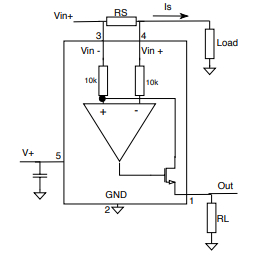
\includegraphics[width=0.65\textwidth]{INA169_setup.jpg}
        \vspace{-5mm}
        \caption{INA169 configuration}
        \label{fig:currentsense}
    \end{figure}
  \end{minipage}
  \hfill
  \begin{minipage}[b]{0.45\textwidth}
    \begin{table}[H]
    \centering
    \begin{tabular}{|c|c|}
    \hline
        \textbf{Rs} & \textbf{Range}\\
        10\ohm  & 3.5mA-35mA\\
        1\ohm   & 35mA-350mA\\
        0.1\ohm & 350mA-3.5A\\
        \hline
    \end{tabular}
    \vspace{5mm}
    \caption{Current sense range.}
    \end{table}
  \end{minipage}
\end{figure}


\newpage
\subsection{MAX485}
The MAX485 is a low power level shifting RS485 transceiver chip which operates from a single 5V supply. The IC contains one driver and one receiver. The receiver has an input has a fail-safe feature that guarantees a logic-high output if the input is open circuit.
\vspace{2mm}

\begin{figure}[H]
  \centering
  \begin{minipage}[b]{0.38\textwidth}
    \centering
      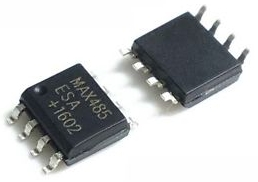
\includegraphics[width=0.6\textwidth]{max485.jpg}
    \caption{MAX485 chip \cite{max485} }
  \end{minipage}
  \hfill
  \begin{minipage}[b]{0.59\textwidth}
    \begin{table}[H]
    \centering
    \begin{figure}[H]
        \centering
        \begin{tabular}{|l|}
        \hline
        \textbf{The MAX485 has the following features:}\\
        - Common-Mode input voltage range from -7V to 12V\\
        - Functions normally from 0°C to 70°\\
        - Allows for up to 32 transceivers on the bus\\
        - Has a data rate of 2.5Mbps\\
        - Current-limiting shutdown protection\\
        - Thermal shutdown protection\\
        \hline
        \end{tabular}
    \end{figure}
    \end{table}
  \end{minipage}
\end{figure}

The data sheet supplies all the information required to run the MAX485 chip, this was used to create the pin setup seen below in Figure 3.12. Which was used when creating the testing methods.
\vspace{15mm}

\begin{figure}[H]
\centering
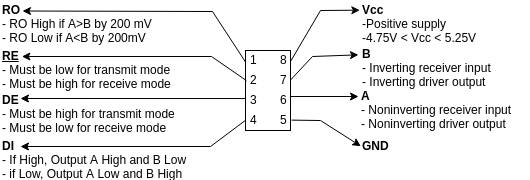
\includegraphics[width=1\textwidth]{MAX485_setup.png}
\caption{MAX485 pin setup}
\label{fig:model}
\end{figure}

\newpage
\subsection{Communication lines}
\vspace{-5mm}
The connector cable used for the communication will be constructed from two wires that twist together over the length of the connection and terminated with termination resistors between the two cables at the beginning and end of each connection. The twisting of the wires is done for the purpose of cancelling out any electromagnetic interference from any external source as well as any noise produced from switch mode power supplies nearby\cite{twisted}.

\vspace{-5mm}
\begin{figure}[H]
\centering
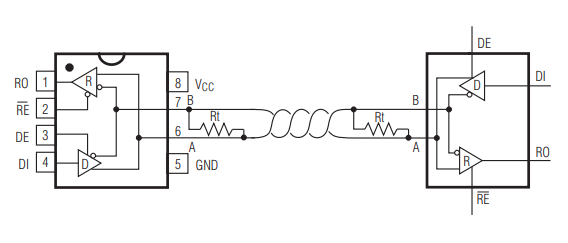
\includegraphics[width=0.6\textwidth]{MAX485_example.png}
\vspace{-7mm}
\caption{Differential communication over the twisted pair \cite{twistedpair}}
\end{figure} 
\vspace{-8mm}
Termination resistors, Rt, are used to match the impedance of a transmission line to the hardware impedance of the interface it is connected to. This allows the the signals to be received with maximum power.  Unterminated, or termination with some value unequal to the impedance of the cable, leads to mismatch that creates reflections in the network. Reflections are part of the energy of the signal that literally returns back up the line. Reflections can constructively or destructively interfere with the next bits propagating down the bus\cite{termination}.

\vspace{-7mm}
\subsection{Connector}
\vspace{-5mm}
The chosen connectors for the servo board had different requirements. The connectors from the buck converter to the servo motor needed to be able the high currents that the motor could draw while the rest of the pins will be used for low current applications. For this, the Molex through hole male pin connectors were chosen which can handle up to 4A.
\vspace{-5mm}
\begin{figure}[H]
\centering
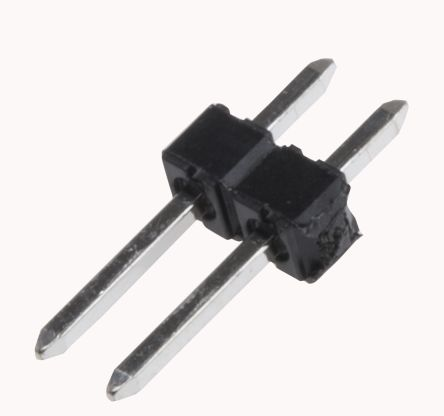
\includegraphics[width=0.3\textwidth]{molex.jpg}
\caption{Molex though hole male pin connector\cite{molex}}
\label{fig:model}
\end{figure} 
\vspace{-5mm}


\newpage
\subsection{Buck Converter}
\vspace{-3mm}
The buck converter chosen for this design needed to output 5V at up to 4 A, with an input voltage range of 5.5-40 Volts. While being small enough to minimise space but big so that it can be still soldered by hand. Using Texas Instruments online power supply designer, Webench. Webench generates the required circuit component values when choosing a buck converter. There were four options where available, seen below in Table 3.4.
\begin{table}[H]
    \centering
    \begin{tabular}{|l|}
    \hline
        1. LM5088 HTSSOP (16 pin) 5.00 mm × 4.00 mm package\\
        2. TPS54561  WSON (10 pin) a 4.00 mm × 4.00 mm package\\
        3. TPS54560 HSOP (8 pin) 4.89 mm x 3.9 mm package\\
        4. LM5145RGYR VQFN (20 pin) 3.50 mm × 4.50 mm  package\\
        \hline
    \end{tabular}
    \caption{Available buck converters}
\end{table}
\vspace{-5mm}
The buck converter chosen was The LM5088, a high voltage non-synchronous buck controller which features all the necessary functions to implement an efficient high voltage buck converter using a minimum number of external components. This Buck controller is typically used for motor driver and USB powered applications. 
\vspace{-2mm}
\begin{figure}[H]
  \centering
  \begin{minipage}[b]{0.4\textwidth}
    \centering
        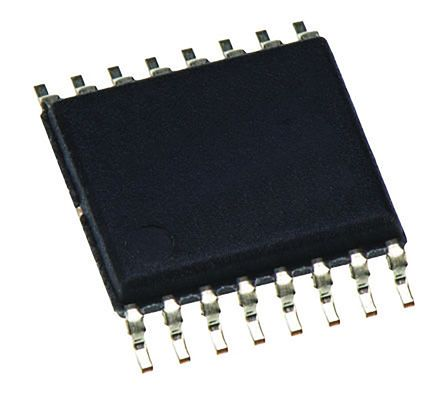
\includegraphics[width=0.45\textwidth]{buck.jpg}
        \caption{LM5088 \cite{buck}}
        \label{fig:model}
  \end{minipage}
  \hfill
  \begin{minipage}[b]{0.55\textwidth}
    \begin{table}[H]
      \centering
        \begin{tabular}{|l|}
        \hline
          \textbf{The LM5088 has the following features:}\\
            - Operates between -40\degree C to 125\degree C\\
            - Input voltage range of 4.5V to 75V\\
            - Thermal shutdown protection\\
            - Adjustable output voltage from 1.205V\\
        \hline
        \end{tabular}
        \caption{LM5088 features}
    \end{table}
  \end{minipage}
\end{figure}
\vspace{-4mm}
A simplified schematic of the typical setup of the LM5088 with all its needed external components can be seen below in Figure 3.16.
\begin{figure}[H]
  \centering
    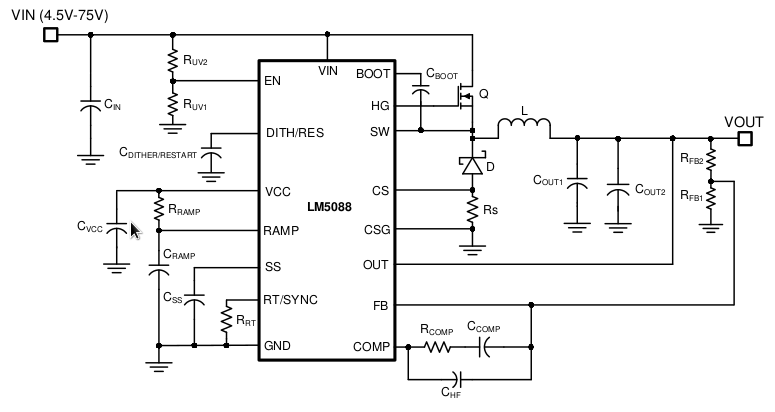
\includegraphics[width=0.6\textwidth]{LM5088_setup.png}
    \caption{LM5088 typical setup}
\end{figure}




\newpage
\subsection{Voltage regulator}
\vspace{4mm}
The voltage regulator chosen needed to be able to regulate the 5V output from the buck converter to the 3.3V needed by the microcontroller to run. The MCP1702 chip is a low power compact chip that only requires an input and output capacitor to run. 
\vspace{4mm}
\begin{figure}[H]
  \centering
  \begin{minipage}[b]{0.4\textwidth}
    \centering
    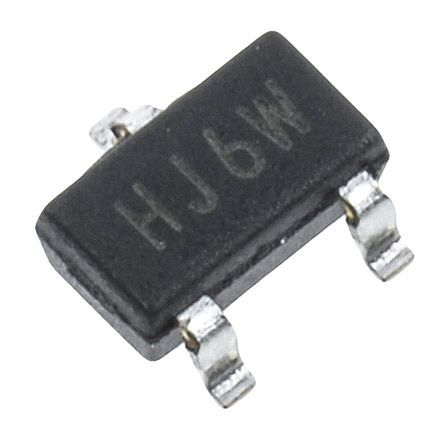
\includegraphics[width=0.4\textwidth]{MCP1702.jpg}
    \caption{MCP1702 chip}
  \end{minipage}
  \hfill
  \begin{minipage}[b]{0.55\textwidth}
    \begin{table}[H]
      \centering
        \begin{tabular}{|l|}
        \hline
          \textbf{The MCP1702 has the following features:}\\
            - Input voltage range of 2.7V to 13.2V\\
            - Output 3.3V with a 0.4\%  tolerance\\
            - Short circuit protection\\
            - Thermal shutdown protection\\
            \hline
        \end{tabular}
        \caption{MCP1702 features}
    \end{table}
  \end{minipage}
\end{figure}
\vspace{5mm}
The MCP1702 is a low dropout (LDO) voltage regulator. Typically used in battery powered applications, smoke detectors as well as digital cameras amongst other devices and applications.
\vspace{5mm}
A simplified schematic of the typical setup of the MCP1702:
\begin{figure}[H]
  \centering
    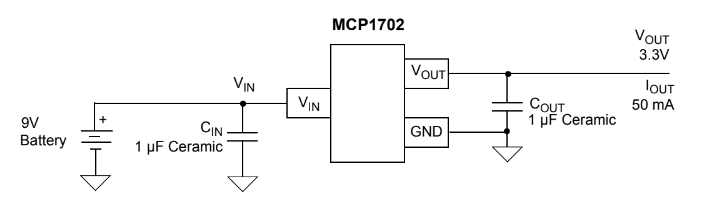
\includegraphics[width=0.8\textwidth]{MCP1702_setup.png}
    \caption{MCP1702 typical setup}
    \label{fig:model}
\end{figure}










 




 
